\chapter{Definitions}
\label{chap:definitions}
This work proposes the application of a high availability technique to a context broker system. For a better understanding of the system and its development, definitions of Context, Context-Aware System, Context Representation, Fault Tolerance and High Availability related terms are presented.

\section{Context}
\label{sec:context}

Context has had many definitions throughout the years. The first definition of Context regarding human-computer interaction related to location, identities of nearby people and objects, and the changes happening to those \cite{schilit1994disseminating}.  Similarly, a later definition sees context as location, people around the user, time of day, season, temperature, etc \cite{brown1997context}. Many authors have also defined context using synonyms, e.g. the idea of “environment”, i.e., what the computer knows about the user's environment \cite{brown1995stick}, or context as user's situation \cite{franklin1998all}. Thus, a lot of definitions have existed, but they all end up being too specific. Context is about the whole situation of an application and its users, and we can't really define it as being too specific to something like a location, or the environment a user is in.

Therefore, looking for a broader definition of context, this work uses the following: ``Context is any information that can be used to characterize the situation of an entity. An entity is a person, place, or object that is considered relevant to the interaction between a user and an application, including the user and application themselves.'' \cite{dey2000providing}.

\subsection{Context-Aware System}
Like context, context-awareness has had several definitions over the years. The first definition restricted it to applications informed about context and applications that adapt themselves to context \cite{schilit1994disseminating}. Later on, synonyms have been used to define a context-aware system: reactive \cite{cooperstock1995evolution}, responsive \cite{elrod1993responsive}, situated \cite{hull1997towards}, context-sensitive \cite{rekimoto1998augment} and environment-directed \cite{fickas1997software}. All these definitions refer to either using or adapting to context, however, a more global definition is needed, covering every interaction with context made by the system.

The definition used in this work aims to be more embracing: ``A system is context-aware if it uses context to provide relevant information and/or services to the user, where relevancy depends on the user's task.'' \cite{dey2000providing}.

A context-aware communication system usually comprises several context management functionalities, where context acquisition and provision are the most important ones. We can divide the system in two main component types: context providers and context consumers; a combination of both is also possible. Given this structure, a small scale system could work with direct communication between context providers and consumers, but when a large scale system is built, network boundaries, mobility and other scaling factors give rise to the necessity of having assisting communication mechanisms, e.g. a broker between the consumers and providers \cite{kian2010federated}.

\subsection{How to represent Context}
Context-aware applications deal with the who's, where's, when's and what's (the activities that are occurring) of entities, and interpret this information to define why a situation is occurring. Then, the designer of the application must decide what to do with the information. Once we have the information available, either through automated sensors or through user's interference, we need to represent it in a way a machine can process and store it \cite{dey2000providing}.

Context can be modeled in many ways, the most relevant options being: key-value, markup scheme, graphical, object oriented, logic based and ontology based models \cite{baldauf2007survey}. As this work is developed following the same core as \cite{crippa2010}, it uses the same context representation model: a markup scheme variation, \textbf{ContextML} \cite{knappmeyer2010contextml}. The network nature of the messages (HTTP messages, in this case) facilitates textual, non graphic model. 

\subsection{ContextML}

ContextML is an XML-based representation schema for context information, where it is categorized into scopes and related to different types of entities. It is designed to be used with REST-based communication between the framework components \cite{knappmeyer2010contextml}. It was created within a project called C-CAST (Context Casting) \cite{ccast}, a collaborative work of many companies, research centers and universities, and its main objective is to evolve mobile multimedia multicasting to exploit the increasing integration of mobile devices with our everyday physical world and environment \cite{crippa2010}. The architecture of the system presented in this work is based on the architecture of the C-CAST Project.

The system consists on three core components: \textbf{Context Provider}, \textbf{Context Consumer} and \textbf{Context Broker}. They use an idea of \textit{entity} and \textit{scope} to represent context information, and communicate through particular types of ContextML messages. Basic definitions of all these components are given below \cite{knappmeyer2010contextml}.

\subsubsection{Context Provider}
A \textbf{Context Provider} (CxP) provides context information of a certain type, e.g. weather, location, activity, etc. It gathers data from sensors, network, user interactions, or other sources. A CxP is specialized in a specific domain of context information (location, weather etc).


\subsubsection{Context Consumer}
A \textbf{Context Consumer} (CxC) queries for and uses context data, e.g. is a context-aware application. A CxC can retrieve context information asynchronously through a subscription method, or by a synchronous method where it requests the Broker for a specific information or for a particular Provider interface, to query the Provider directly.

\subsubsection{Context Broker}
A \textbf{Context Broker} (CxB) is the central component of the architecture, and is the focus of this work. It handles and aggregates context information, and is an interface between the other architecture components. The CxB allows CxCs to subscribe to context information, and CxPs to provide this information. It also provides a lookup service, where the CxCs can query the CxB for CxPs that have a particular capability, depending on the CxC’s interest.

\subsubsection{Entity and Scope}
An entity is the subject of interest which context data refers to, and it is composed of two parts: a type and an identifier. The type refers to the category of the entity: username for human users, imei for mobile devices, room for a room with sensors, etc. The identifier specifies a particular item within a set of entities of the same type.

A scope is a set of closely related context parameters. Every context parameter has a name and belongs to only one scope. The parameters of a scope can only be requested, updated, provided and store at the same time, making the data always consistent. For example, a scope \textit{position} has latitude, longitude and accuracy attributes; any operation on this scope is performed on all these attributes: if the latitude is updated, so is the longitude and accuracy, what is correct, because otherwise it would not make sense. Entity-scope association is illustrated in Figure \ref{fig:entityscope}. \par

\begin{figure}
	\centering
	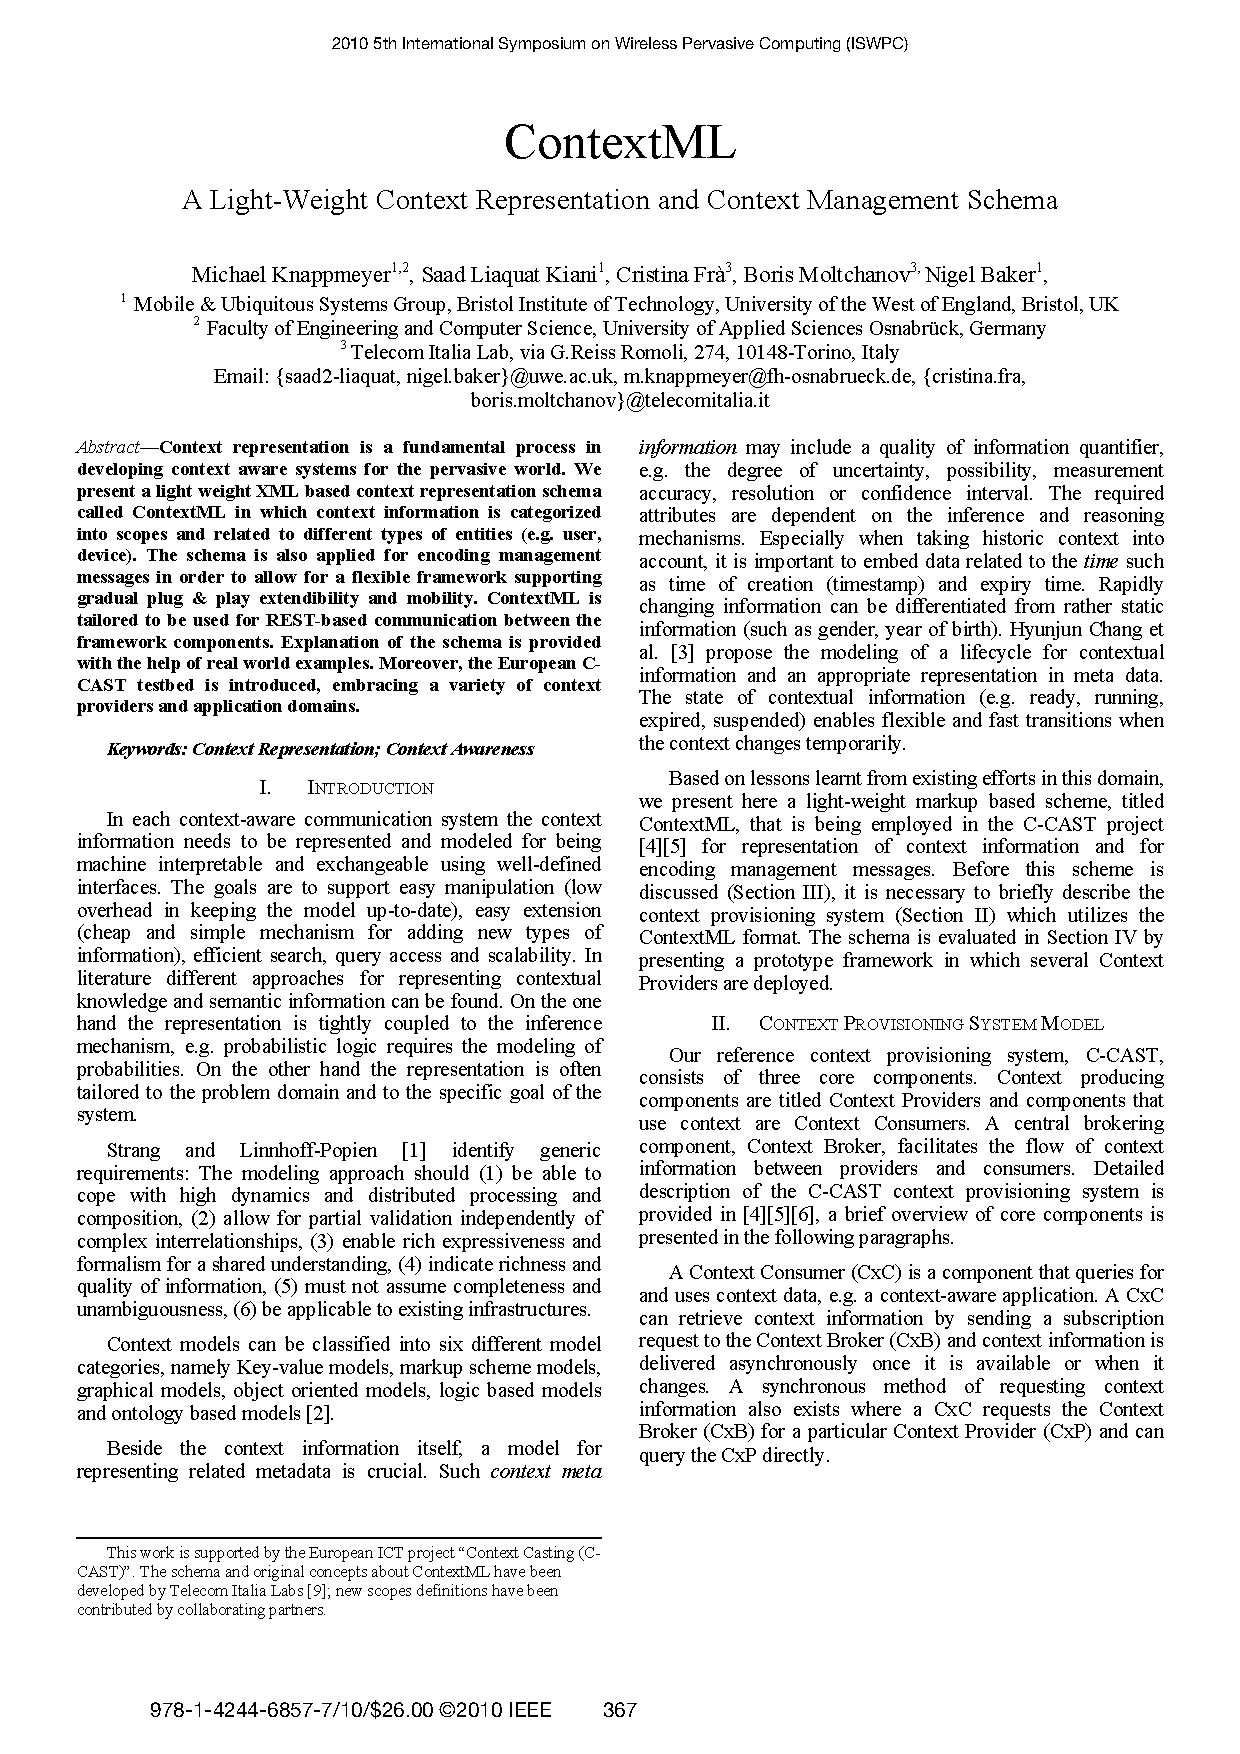
\includegraphics[scale=1]{entityscope.pdf}
	\caption{Entity and Scope relationship}
	\label{fig:entityscope}
	\cite{knappmeyer2010contextml}
	
\end{figure}

\subsubsection{ContextML Messages}
Within the architecture of the system, context is registered, updated and queried following a set of pre-defined ContextML messages \cite{knappmeyer2010contextml}. The ContextML message types used in this work and their usage are shown below, as well as a simple example of each one.

\begin{description}
\item[Advertisement Message]\hfill \\
An Advertisement Message is used by the Context Provider to register its capabilities to the broker. It informs the CxP’s access url (urlRoot), what scopes it supports (scopes), its identifier (name), and optional information about the CxP’s location. An example of a Advertisement Message can be seen in Figure \ref{fig:advertisement}.

\begin{figure}
	\centering
	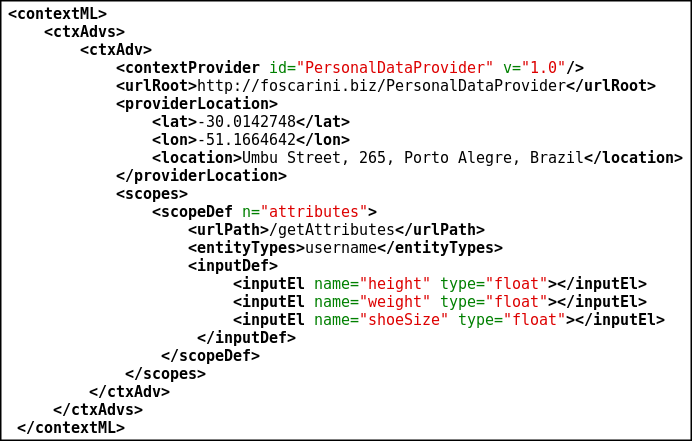
\includegraphics[scale=0.5]{advertisement.png}
	\caption{Provider Advertisement example message}
	\label{fig:advertisement}
	
\end{figure}

\item[CxP Lookup Message]\hfill \\
When a CxC wants to know where it can find a specific scope, it can query the CxB about which of the registered Providers has the desired information. The Broker replies with a ContextML message, describing the Providers that match with the data required by the CxC. An example can be seen in Figure \ref{fig:providers}.

\begin{figure}
	\centering
	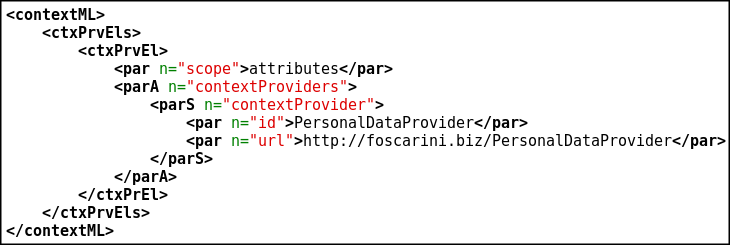
\includegraphics[scale=0.5]{providers.png}
	\caption{Providers Lookup example message}
	\label{fig:providers}
	
\end{figure}

\item[ACK Message]\hfill \\
Acknowledgement is a control message that confirms the execution of various management actions (e.g. advertisement, context update). Each ACK message contains the status of the operation, the HTTP response code, and the identification of the method it corresponds. It also has optional fields to inform scope and entity information. An example is shown in Figure \ref{fig:acknack}.

\begin{figure}[h]
	\centering
	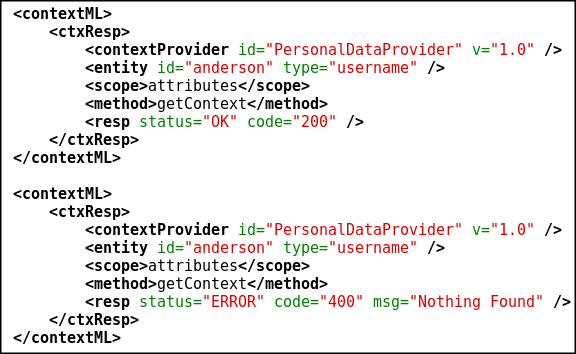
\includegraphics[scale=0.5]{acknack.png}
	\caption{ACK and NACK example messages}
	\label{fig:acknack}
	
\end{figure}


\item[Context Representation Message]\hfill \\
This is the form of representing context data in the architecture. When a Consumer requests or subscribes to a context scope, it receives a ContextML message with the element \textit{‘ctxEl’}, when the information queried is available. \textit{ctxEl} contains information of the provider that has the context queried (contextProvider), the entity and scope it is related to, and the context data in the \textit{dataPart} element. \textit{par}, \textit{parS} and \textit{parA} are constructors to store name-value pairs and attribute collections (structs and arrays) respectively. Every context information that is exchanged is tagged with a \textit{timestamp} (time of its generation) and an expiration time \textit{expires} (validity of the context information), after which the information is considered invalid. An example of a Context Representation Message is shown in Figure \ref{fig:ctxels}.

\begin{figure}
	\centering
	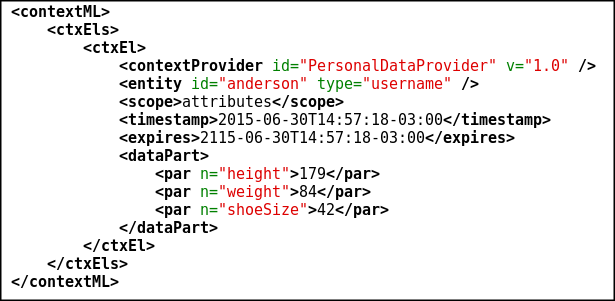
\includegraphics[scale=0.5]{ctxels.png}
	\caption{Context Element example messages (update)}
	\label{fig:ctxels}
	
\end{figure}


\end{description}

\subsection{Overview of Context Data representantion}

In Figure \ref{fig:contextdatadiagram} an overview of how context data is represented in the system is shown. Each element is tied by entity ID, entity type and scope. Each one belongs to only one provider, and has timestamp, expiration data and location information. It can store as many pairs of name and value as it needs, e.g. a location data has pairs of latitude, longitude and accuracy values.

\begin{figure}[h]
	\centering
	\includegraphics[scale=0.5]{contextdatadiagram.png}
	\caption{Context Data representation}
	\label{fig:contextdatadiagram}
	
	\end{figure}



\section{Dependability}
\label{sec:fault_tolerance}

The dependability of a system is the ability to avoid service failures that are more frequent and more severe than is acceptable, i.e., failures will eventually happen, and the system will try to avoid them compromising the correctness of the service. Dependability is an integrating concept that encompasses the following attributes \cite{avivzienis2004basic}:
\begin{itemize}
	\item{Availability:} readiness for correct service
	\item{Reliability:} continuity of correct service
	\item{Safety:} absence of catastrophic consequences on the user(s) and the environment
	\item{Integrity:} absence of improper system alterations
	\item{Maintainability:} ability to undergo modifications, and repairs
\end{itemize}

\subsection{Fault Tolerance}
Many means can be developed to attain the various attributes of dependability and security. Those means can be grouped into four major categories \cite{avivzienis2004basic}:
\begin{itemize}
	\item{Fault Prevention} means to prevent the occurrence or introduction of faults
	\item{Fault Tolerance} means to avoid service failures in the presence of faults
	\item{Fault Removal} means to reduce the number and severity of faults
	\item{Fault Forecasting} means to estimate the present number, the future incidence, and the likely consequences of faults
\end{itemize}

Fault prevention and fault tolerance aim to provide the ability to deliver a service that can be trusted. This work focuses on \textbf{fault tolerance}, which is aimed at failure avoidance, and is carried out via error detection and system recovery.



\subsection{High Availability}
Looking at the dependability attributes described on the previous section, one that this works proposes is implemented in a Context Broker system is availability.

Any loss of service, whether planned or unplanned, is known as an \textbf{outage}. 
\textbf{Downtime} is the duration of an outage measured in units of time (e.g. minutes or hours) \cite{weygant2001clusters}.

A system is expected to be highly available when life, health and well-being, including the economic well-being of a company, depend on it. But even the most highly available services often face outages. In these cases, the expected action is that the service gets completely restored as quickly as possible, with all its capabilities ready to operate.

Availability is measured from the user's point of view. A system is available if the user can use the application he needs \cite{piedad2008high}. The level of availability desired for a system depends on its usage.

Availability is important for systems that require that its services are available for clients for most part of its lifetime, e.g. a web commerce system should not have an extended downtime, as money is lost on possible transactions; or a financial institution, who needs to be able to transfer funds at any time of the day, seven days a week. Some systems may also require a different approach to high availability: a window of service, for example a system that needs to be up for the entire daylight-hours, and can go under maintenance at night, reserving this time to some recovery for example, in case of an outage.

One example of use of a highly available Broker is one that receives temperature values from sensors distributed on a building, concerning fire prevention. It is important that the Broker system is always available, as the information it stores is crucial. Another example is a Broker that stores position information from sensors on a mountain, and ha

High availability solutions are based on system component redundancy. If a component fails, the system is able to continue to operate using a redundant component \cite{engelmann2005concepts}. When looking for a highly available system, many solutions exist, involving replication and redundancy \cite{oraclereplication}, clustering \cite{oracleclustering}, etc.


However, when designing a highly available system, some problems may arise. Single point of failure \cite{engelmann2005concepts}, membership problem \cite{cristian1991reaching}, split-brain \cite{barreradesign}, agreement on distributed transactions \cite{guerraoui2002non}, among others, are well-known and documented problems. Whoever is responsible for the design of the system must take action on avoiding these, to reach an optimal solution.



\subsection{High Availability on Clusters}
This work uses ideas from highly available Cluster systems to structure the Broker system. For that, basic definitions needed to provide the complete understanding of the system are presented.

\subsubsection{Cluster goals}
A cluster is a collection of computer nodes that work
together to provide a much more powerful system. To be
effective, the cluster must be as easy to program and manage as a single large computer. Clusters have the advantage that they can grow much larger than the largest single
node, they can tolerate node failures and continue to offer
service, and they can be built from inexpensive components \cite{barreradesign}.

Some general goals of a Cluster \cite{barreradesign}:
\begin{itemize}
	\item[Commodity] a cluster runs on a collection of off-the-shelf computer nodes interconnected by a generic network 
	\item[Scalability] adding applications, nodes, peripherals,	and network interconnects is possible without interrupting the availability of the services at the cluster
	\item[Transparency] a cluster presents itself as a single system to clients outside the
	cluster. Client applications interact with the cluster as if it were a single high-performance, highly reliable server. The clients as such, are not affected by interaction with the cluster and do not need modification
	\item[Reliability] ability to detect failures of the hardware and software resources it manages
\end{itemize} 

We can use abstractions of nodes and resources in clusters, as nodes being communicate via messages over network interconnects, and use communication timeouts to detect node failures; and a resource represents certain functionality offered at a node \cite{barreradesign}.

In short, a Highly Available Cluster consists of multiple machines interconnected by a common bus \cite{azagury1994highly}.

\subsubsection{Nonblocking protocols}
Protocols that allow operational sites to continue transaction processing even though site failures have occurred are called nonblocking \cite{skeen1981nonblocking}.

Crash recovery algorithms are based on the notion that certain basic operations on the data are logically indivisible. These operations are called transactions.

The processing of a single transaction is viewed as follows. At some time during its execution, a commit point is reached-where the site decides to \textit{commit} or to \textit{abort} the transaction. A commit is an unconditional guarantee to execute the transaction to completion, even in the event of multiple failures. Similarly, an abort is an unconditional guarantee to ''back out'' the transaction so that none of its results persist. If a failure occurs before the commit point is reached, then immediately the site will abort the transaction \cite{skeen1981nonblocking}.

One can find a wide variety of nonblocking protocols, e.g. two-phase (prepare and commit), three-phase (prepare, pre-commit, commit) protocols \cite{skeen1981nonblocking}. This work uses as inspiration a three-phase commit protocol variation shown in \cite{guerraoui2002non}.

 